%!TEX root = thesis.tex
%% %% ***************** Research materials and methods *****************

%% ************************************************ 3 ************************************************

\section{Research material and methods}\label{sec:research-material-and-methods}
%\section{Tutkimusaineisto ja -menetelmät}

In the next section
we explain in more detail
what the data used in the study
consists of
and what methods were used
in attempt to answer the research goals.
The content of the section is briefly described below,
and the steps of the research are explained.

The data in the research is mainly made of two parts.
The most important part is, obviously,
the log data produced by the numerous RPA processes.
The second data part,
complementing the study,
is the support ticket data written by clerks of customer banks.
In order to use the data safely in the cloud environment
it was necessary to sanitize the data
from any sensitive information.
This was done by anonymizing the log data
and using only timestamps from the support tickets.

After confirming the results of anonymization,
the data was preprocessed into a better form
to make it more usable by algorithms.
More processing was done inside the pipeline
as ML Studio offered several usable components for this
but main cleaning was easier and to execute in local environment.
This was also done with PowerShell scripting.

The actual ML pipeline structure
is discussed in the next section.

%% ************************************************************************************************************

\subsection{Support ticket data}\label{subsec:meth-efecte-ticket-data}

Like all other software,
RPA components fail from time to time.
As described before,
RPA logs are verbose
making possible error identification from among them hard.
Due to that,
it is not feasible to create log parsers
that would be able to identify critical errors
from within thousands of lines of log.
When critical error happens
causing the RPA process to fail,
the banking clerks need to finish manually
the job left by the RPA robot.
Every time this happens,
these clerks then send a support request ticket
to Samlink technical help desk
and ask to fix the issue.

When clerks send the ticket to technical support
a verbose description of the situation is written
to help developers to identify the problem.
This description often contains sensitive end customer information
like bank account details and social security numbers.
To avoid privacy issues when processing this data,
it was decided to use only timestamps of the tickets.
The resulting data was practically a list of date and time values.
More about the issue from privacy point of view
is described in section~\ref{subsec:meth-data-anonymization}.

%% ************************************************************************************************************

\subsection{RPA log data}\label{subsec:meth-rpa-log-data}
Robotic process algorithms used in Samlink
are designed to ease the workload of bank clerks.
RPA robots work in behalf of bank clerks
executing routine tasks that require mostly manual labor.

Like other software,
RPA also produces log data during runtime.
As dozens of RPA automations are running
in several bank environments
the amount of log entries produced is also significant,
up to over a million lines per week.
This log data is not in consistent structure
as it is formed out of typical CSV data
and injected with even more inconsistent JSON data
that varies in contents vastly.
\todo{refer to appendices, include examples of data}

RPA log data is stored in SQL database.
The database is split in live production log
that is gathered for two weeks
and then moved to archive that has
several years worth of log.
In this study we used archived data
as it was easier to acquire in one run
without the need to merge different parts together.
Archive also had data
that was considered as sufficient amount
for machine learning algorithm training,
with data entries spanning almost two and a half years
and rowcount exceeding 80 million.

%% TODO: Discuss about rawmessage memory issues in result section!

%% TODO: check below to make sense
Samlink RPA logs have few standard fields.
These are listed in a table below~\ref{tab:log-row-fields}.
The most notable aspect of these fields
are the \textit{message} and \textit{rawmessage} fields.
\textit{Message} holds the short log message
written by the RPA agent during automation execution.
This includes details about the issue,
what part of the process failed,
and possible stack trace of the error.

\textit{Rawmessage} is JSON-formatted representation
of all the default features,
including the message
and multiple other additional features
that RPA agent is able to output regarding the execution.
These additional fields are what vary from log entry to log entry.
Some of the possible fields are shown in a table~\ref{tab:log-row-fields},
but several other field types exist,
and the JSON data in them can be nested in multiple layers.

Without rawmessage,
the data was in pure CSV-format.
However,
it was not certain
that rawmessage would not hold usable data for ML~.
In the end,
the usage of rawmessage was not studied in satisfying extent
as it demanded too much resources in ML Studio to process.

%% TODO:!! below:
% In the data preprocessing phase the rawmessage was kept along
% and it lead to some interesting and most likely reusable preprocessing scripts.

\begin{table}[]
    \centering
    \begin{tabular}{|L{0.25\textwidth}|L{0.25\textwidth}|L{0.5\textwidth}|}
        \hline
        \textbf{Field}    & \textbf{Contents}                               & \textbf{Examples}                                                             \\ \hline
        organizationUnitId & Samlink organization unit                       & 5                                                                            \\ \hline
        level              & Log level                                       & Information | Warning | Error | etc.                                         \\ \hline
        logType            & Type of log entry                               & Default | User                                                               \\ \hline
        timeStamp          & Date and time for log entry                     & 2019-09-10T03:00:01.6278373+03:00                                            \\ \hline
        fingerprint        & Unique identifier for log entry                 & bcd51984-agdc-40a6-b571-y6a97f98a4e3                                         \\ \hline
        machineName        & Workstation name of the RPA agent               & T2490A1011                                                                   \\ \hline
        processName        & Name of the RPA automation                      & RPA-bank-hakemusten-tietojen-siirto\_Samlink Production                      \\ \hline
        jobId              & Identifier for current RPA automation execution & 24a84531-010b-457f-90t1-5ayc98d7b557                                         \\ \hline
        robotName          & Name of the agent executing automation          & RPA-BANK-1-1234                                                              \\ \hline
        machineId          & Workstation ID number                           & 5                                                                            \\ \hline
        message            & Short message regarding the entry               & Throw exception: Saldo ei riitä | \newline Tarkistettiin A:n nimi                    \\ \hline
        rawmessage         & JSON formatted message including most of the above columns and several more fields regarding the log entry &
        \{
        \textbf{"message"}: "Siirryttiin Varallisuus-sivulle.",\newline
        \textbf{"level"}: "Information",\newline
        \textbf{"logType"}: "User",\newline
        \textbf{"timeStamp"}: "2019-09-10T03:00:50.6103121+03:00",\newline
        \textbf{"fingerprint"}: "70f44345-22bb-46df-885e-75f180fc4d48",\newline
        \textbf{"windowsIdentity"}: "LOCAL\textbackslash{}\textbackslash{}T123456",\newline
        \textbf{"machineName"}: "T2490A1011",\newline
        \textbf{"processName"}: "RPA-bank-hakemusten-tietojen-siirto\_Samlink Production",\newline
        \textbf{"processVersion"}: "1.0.7111.31245",\newline
        \textbf{"jobId"}: "24a84531-010b-457f-90t1-5ayc98d7b557",\newline
        \textbf{"robotName"}: "RPA-BANK-1-1234",\newline
        \textbf{"machineId"}: 11,\newline
        \textbf{"fileName"}: "LisaaTiedot\_Talous\_Varat",\newline
        \textbf{"logF\_BusinessProcessName"}: "rpa-sp-011-OTT-valmistelu"  \}
        \\ \hline
    \end{tabular}
    \caption{Log fields in RPA log data}
    \label{tab:log-row-fields}
\end{table}

\todo{Maybe some more info about the log data? Open up the table?}

%% ************************************************************************************************************

\subsection{Data anonymization}\label{subsec:meth-data-anonymization}

\subsubsection*{Support ticket data privacy}
Samlink handles highly sensitive banking customer data in its processes,
such as personal identification numbers, home addresses, email addresses and bank account numbers.
All possibly sensitive data had to be removed
before data could be transferred out from production environment to cloud.
Due to bureaucratic reasons,
technical support tickets were under more strict policies.
Because of this,
they were allowed to be used in the research
on condition that no business critical nor customer sensitive information
was processed in the first place.
Only way to assure this
was to select solely timestamp fields from ticket data.
Thus, no sanitation for ticket data was needed
as ticket data consisted of only list of datetime values.

%% ............................................................................................................

\subsubsection*{RPA log data sanitization}
Information privacy is one of the key values in Samlink business promise
as company develops high security banking applications
and processes sensitive customer data.
Thus, several aspects were needed to take into consideration
before log data could be authorized for thesis study usage.
To improve privacy,
it was decided to assume
that personal customer details are not critical information
for ML algorithm training
if goal is to find possible problems in RPA runtime
and not detect individual customer related problems.
This way it was not necessary to achieve adequate security
by less secure and more effort consuming ways
such as pseudonymization or k-anonymization
(explained in the section \ref{subsec:bg-data-sensitivity}), %% TODO: Check it's explained
which would have also required strict inspections
before data could have been approved for cloud processing.
\todo{References?}

As production environment is built on Microsoft Server based solution,
and because it was highly unrecommended
to install additional software to the production server,
data acquiring and anonymization tools were chosen
based on what was already usable in the RPA production environment.
Microsoft PowerShell offers sufficient tools
for database SQL querying
and stream editing.
The amount of data was significant
which made straight file editing impossible
due to the memory limitations.
Thus, stream editing was necessary
for finding and replacing
sensitive information from the data.
\todo{maybe references?}
%% TODO: References!

Anonymization took good proportion of the time in workdays
as processes were slow,
the amount of data was huge
and multiple re-runs were needed
before the results were seemed adequate.
\todo{Appendix of the script used. Does this need more explaining?}
%% TODO: appendix of the script used

%% TODO: add more details about regex and features anonymized

%% ************************************************************************************************************

\subsection{Data formatting}\label{subsec:meth-data-formatting}
At the beginning of the research,
the log data from RPA was in SQL database.
However,
the database used was not "pure"
in a way that typical relational databases are,
but some columns included JSON-formatted data in them.
For ML algorithms to be able to read the given data with ease
this kind of impurities needed to be cleared from the data.

When feeding the log data to anomaly detection algorithm,
it was necessary that all the rows were as minimally unique as possible
in order to use the pattern finding abilities of the algorithm.
Too unique data points would have made all of them anomalies
compared to each other.
Thus, all unique features were stripped from the data,
such as the fingerprint value
that was unique for each data point.
As rawmessage-field included data in textual JSON form
that identified unique automation executions at some extent,
it was processed with additional script
which removed manually such field values.
These fields were
timestamp, fingerprint, and job ID values.
When training ML algorithm with rawmessage,
timestamp and job ID values were included
from their corresponding fields outside rawmessage.

%% TODO:
\todo{Add reference to appendices}


%% ************************************************************************************************************

\subsection{Azure cloud resources}\label{subsec:meth-azure-cloud resources}

\todo{This section is under construction! Here are some things we are discussing here:}
\begin{itcomment}
    Azure resources, such as virtual networks, storage spaces, connections to ML studio \etc

    What kind of resources were usable based on the issue at hand
    and limitations by the company (cost, basically).
    We discuss some things about Azure ML Studio
    but only in extent of what parts needed configuring.
\end{itcomment}

%% TODO: <Azure resources, virtual network etc.>
%% TODO: Azure architecture

Azure provides a vast set of tools and resources
for different kinds of cloud projects.
Resources needed for Azure ML Studio usage
depends on the subscription used
and security restrictions set by subscription administrators.
When starting this study,
due to these restrictions,
all resources used for ML training in this project
needed to be inside the same virtual network.
Azure ML Studio environment could be opened from any network,
but most of the features were unavailable
if computer browsing studio UI was outside this virtual network.
Thus,
a virtual machine had to be acquired as Azure resource
from within the same network as other resources
and ML Studio UI had to be opened with the browser on this machine.
Later on it was found
that Azure Machine Learning Workspace networking feature
could be configured to allow public access
making possible to access ML Studio UI from all networks.


%% TODO: explain picture
\todo{Explain picture}

\begin{figure}[htb]
    \centering
    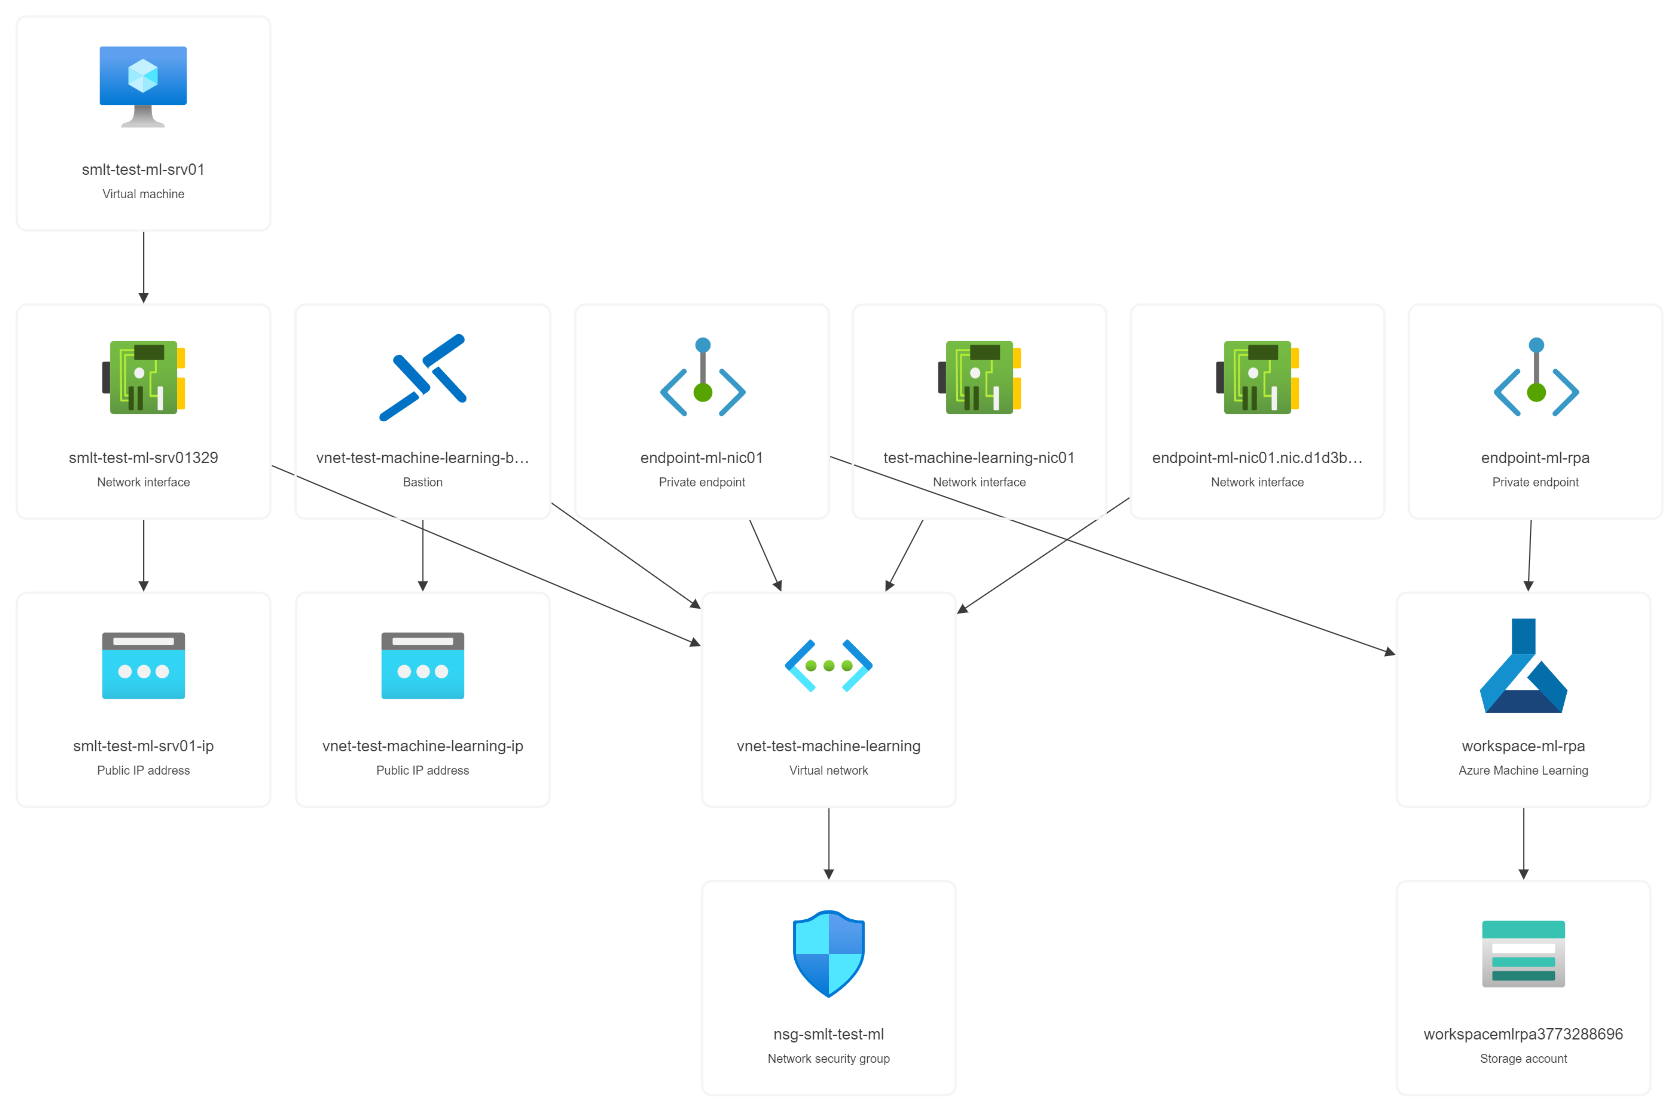
\includegraphics[width=\textwidth]{./appendices/azure-resource-diagram}
    \caption{Azure cloud resources needed and their relations
    \label{fig:azure-diagram}}
\end{figure}

%% ............................................................................................................

\subsection{Azure ML Studio}\label{subsec:meth-azure-ml-studio}

During the initial pipeline runs
the execution came to an abrupt stop
and Azure notified about memory issues. %% TODO: Add reference to issue
These problems were linked to the data amount
which had to be reduced to 600 megabytes
before any pipeline could be finished using the data.
This reduction was against the initial goal
where preferably all the data could have been used.

Considerable amount of time was used
to fix or avoid this issue
but nothing clear was found
that would explain the error received.
While working with the issue
it was also noted
that data needed more cleaning
in order to ease the preprocessing phase
as described with more detail in section~\ref{subsec:meth-data-anonymization}
Thus,
the data had to be imported from log archive
and anonymized once more.

To advance the study more efficiently
it was decided to trim info-type log messages from data
hence reducing the data amount considerably.
Final data included 8.6 million log rows
which was about 10\% of the original data size.
Before final cleaning operations
the data took 8.1GB od disk space,
and after cleaning the rawmessage-field
the final disk size was 6.6GB\@.
Even with this data size,
some Azure ML components faced this memory issue
and forced us to choose such components
that were able to handle these data amounts.

%% TODO: Move some parts of the above memory problem elsewhere

In addition to the data we used to train the algorithm,
we needed to set up computing instance
in Azure ML studio.
Some predefined resource limitations
affected the computing instance choosing
and the memory issue encouraged us
to pick memory prioritized instances.
Single computing instance did not work,
but we needed to choose a computing cluster instead
to be able to run ML training pipeline.
%% TODO: Maybe what other choises were possible?

%% TODO: Data stores etc?

\todo{Some more info about the resources needed}


\clearpage